\documentclass[conference]{IEEEtran}
\IEEEoverridecommandlockouts
\usepackage[spanish]{babel}
\usepackage{cite}
\usepackage{pgfopts}
\usepackage{amsmath,amssymb,amsfonts}
\usepackage{algorithmic}
\usepackage{graphicx}
\usepackage{textcomp}
\usepackage{xcolor}
\def\BibTeX{{\rm B\kern-.05em{\sc i\kern-.025em b}\kern-.08em
    T\kern-.1667em\lower.7ex\hbox{E}\kern-.125emX}}

\begin{document}

    \title{Métodos de  Programación Orientada a Objetos.\\
        Polimorfismo\\
        {\footnotesize Practica Cinco}}
    \author{\IEEEauthorblockN{Ortega Ezquerra, Jesús Rodigo}
        \IEEEauthorblockA{\textit{Ingeniería Eléctrica y Electrónica.} \\
        \textit{Univesidad Nacional Autónoma de México}\\
        CDMX, México \\
        jeroorez@gmail.com\\
        https://orcid.org/0000-0002-8965-1189}
        \and
        \IEEEauthorblockN{Morales Medina, Antonio}
        \IEEEauthorblockA{\textit{Ingeniería Eléctrica y electrónica.} \\
        \textit{Univesidad Nacional Autónoma de México}\\
        CDMX, México \\
        moralesmedinaa201@gmail.com}
    }\maketitle

    \begin{abstract}
        En esta práctica se busca entender el uso del polimorfísmo en el lenguaje 
        de java para la clase de Modelos de Programación Orientada a Objetos.
    \end{abstract}
    
    \begin{IEEEkeywords}
        POO, java 8, polimorfismo, instenceof, abstract, extends, super
    \end{IEEEkeywords}

    \section{Introducción.}

        Para el previo de esta práctica se debían preparar tres clases:
    
        \begin{enumerate}
            \item Poligono(superclase)
            \item Triangulo
            \item Cuadrilatero
        \end{enumerate}
    
        \begin{figure}[htbp]
            \centerline{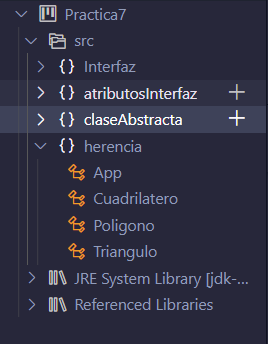
\includegraphics[scale=0.8]{./pics/1}}
            \caption{Estructura del paquete herencia.}
            \label{fig}
        \end{figure}

        La clase \texttt{App} se escribió en clase cómo \texttt{MPOOP7}  para efectuar las actividades uno y dos 
        \subsection{Objetivos.}
            \begin{enumerate}
                \item Analizar la herencia y privacidad de clases base así como sus derivadas para relacionar sus instancias que la llevan a ser polomórficas.
                \item Definir el funcionamiento de el método \texttt{instanceof} y conocer la instancia de los objetos creados.
                \item Reconocer la diferencia de una clase abstracta y una privada
                \item Conocer las interfaces en Java para su implementación.
            \end{enumerate}
    
        \section{Clases base.}
    
        \begin{quote}
        ''El concepto de herencia conduce a una estructura jerárquica de clases o estructura de árbol, lo cual significa que en la OOP todas las relaciones entre clases deben ajustarse a dicha estructura.'' \cite{IEEEexample:ProgramacionConJava}
        \end{quote}

        \subsection{Tipos de clase.}

        \begin{enumerate}    
            \item \textit{Clase Base}\\
                También llamada clase padre o superclase, es aquella que va a heredar a las clases hijas que derivan a partir de la clase padre. (Figura \ref{fig1})
            \item \textit{Clase Derivada}\\
                Clase que reinstancía a la clase padre de la que deriva para ser una de sus subclases, cabe mencionar que hereda los métodos y variables de la clase padre.
                Se le conoce también como clase hija o subclase.
        \end{enumerate}
        
        \begin{figure}[htbp]
            \centerline{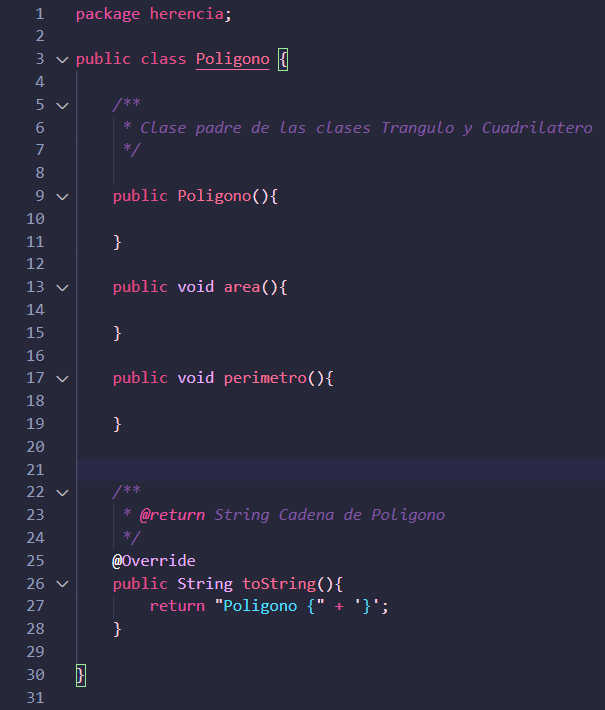
\includegraphics[scale=0.3]{./pics/2}}
            \caption{Superclase Poligono.}
            \label{fig1}
        \end{figure}

        \subsection{Actividad uno.}
        
            Se crea un objeto llamado \texttt{poligono} y se imprime la cadena de atributos.
            se crea otro objeto llamado \texttt{objeto} y se asocia a la clase arbol de java \texttt{Object.lang} y cuando se intenta imprimir en pantalla nos regresa la dirección de memoria dónde se encuentra almacenado \texttt{objeto} 
            En cambio, cuando se asocia con la clase padre \texttt{poligono} que contiene el método \texttt{toString();} es cuando envía correctamente los valores de su clase en forma de cadena.Figura \ref{fig2}

            \begin{figure}[htbp]
                \centerline{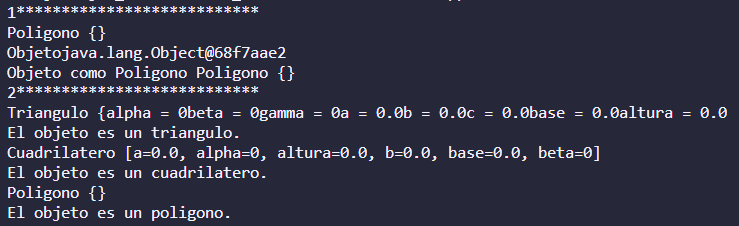
\includegraphics[scale=0.35]{./pics/3}}
                \caption{Actividad uno y dos en consola.}
                \label{fig2}
            \end{figure}

        \subsection{Actividad dos.}

            Para la actividad dos se asocia a cada una de las clases para darle la característica de polimorfismo.

    \section{Método instanceof.}
        \medskip
        \subsection{\texttt{Instanceof}} 
        
            \begin{quote}
                "The instanceof keyword compares an object to a class or interface type.It also looks at subclasses and subinterfaces. x instanceof Object returns true unless x is null" \cite{IEEEexample:OCPJSE}
            \end{quote}

            \medskip{}
    
            Lo que hace el método \texttt{instanceof} es comparar el objeto de una clase o interfaz. También se utiliza para subclases y subinterfaces.
            Para la actividad uno, usaremos la clase poligono cómo clase padre para extender otras figuras geométricas. (Figura \ref{fig3})

            \begin{figure}[htbp]
                \centerline{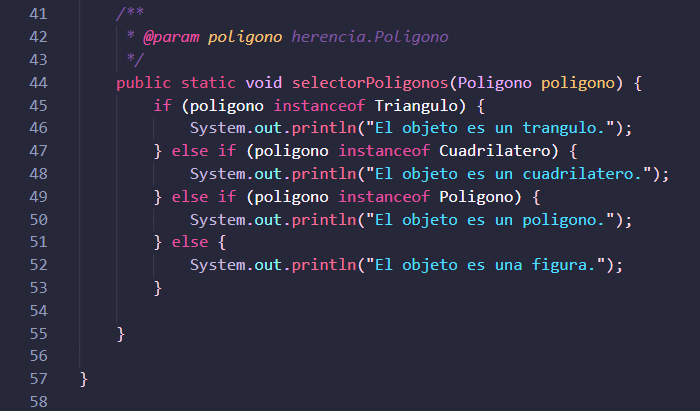
\includegraphics[scale=0.35]{./pics/4}}
                \caption{Condicional anidada con el el método instanceof.}
                \label{fig3}
            \end{figure}

    \section{Clase abstracta.}

        \medskip
        
        \subsection{\texttt{abstract}}
            
            \begin{quote}
                {''In software engineering and programming language theory, the abstraction principle (or the principle of abstraction) is a basic dictum that aims to reduce duplication of information in a program (usually with emphasis on code duplication) whenever practical by making use of abstractions provided by the programming language or software libraries. The principle is sometimes stated as a recommendation to the programmer, but sometimes stated as requirement of the programming language, assuming it is self-understood why abstractions are desirable to use.''} \cite{IEEEexample:JavaAbstraction}
            \end{quote}
        
            \medskip{}

            En pocas palabras, la abstracción es una forma de ahorrar espacio en memoria así como líneas de código.

        \subsection{Actividad tres.}

        \begin{figure}[htbp]
            \centerline{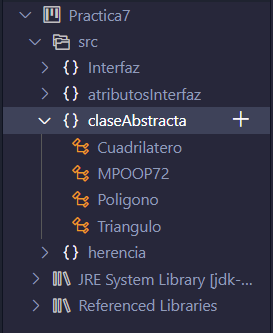
\includegraphics[scale=0.4]{./pics/5}}
            \caption{Arbol de jararquía de claseAbstracta.}
            \label{fig4}
        \end{figure}

        Esta vez se hace exactamente lo mismo que el paquete de \texttt{herencia} (Figura \ref{fig4}), sólo que a diferencia de la actividad uno y dos, en la actividad tres su modificador de acceso se declara cómo \texttt{abstract} para analizar su comportamiento. (Figura \ref{fig5})
            
        \begin{figure}[htbp]
            \centerline{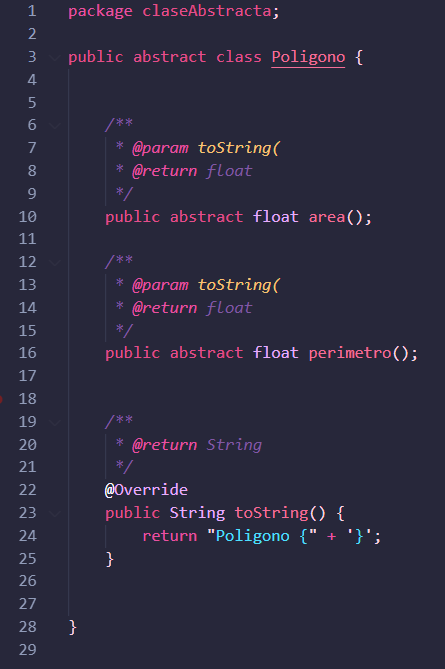
\includegraphics[scale=0.4]{./pics/6}}
            \caption{Poligono para claseAbstracta.}
            \label{fig5}
        \end{figure}
            
        Observamos que las clases abstractas no se pueden instanciar pero sus sublases si lo hacen.(Figura \ref{fig6})

        \begin{figure}[htbp]
            \centerline{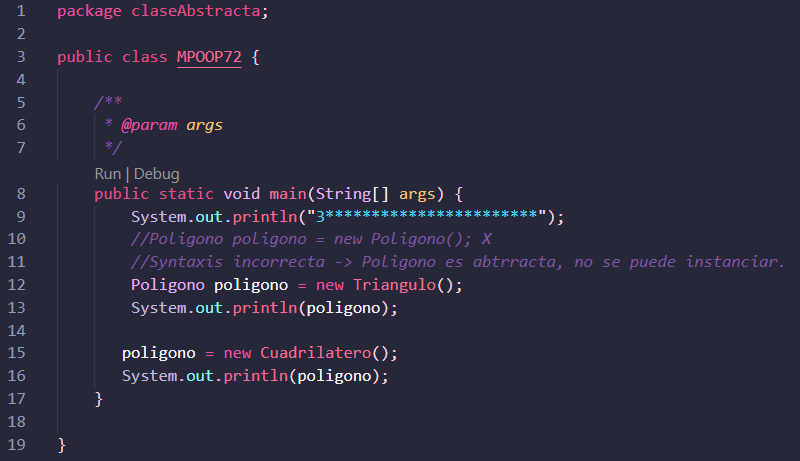
\includegraphics[scale=0.35]{./pics/9}}
            \caption{Main para claseAbstracta.}
            \label{fig6}
        \end{figure}

        Algunos autores se reducen a definir una clase abstracta cómo aquella que no sabremos como emplear, pero obligatoriamente debe estar ahí.
        Una clase abstracta podría ser aquella que permite generar sublases que en cierto modo van a compartir métodos o parámetros.(Figura \ref{fig7})
        Al final la abstracción de una clase es encontrar una clase arbol que sabremos que derivará en subclases con distintos parámetros que podrían o no comprtir sus parámetros y clases, sean estas abractas o privadas. 
        
        \begin{figure}[htbp]
            \centerline{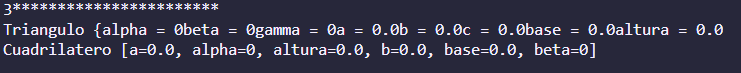
\includegraphics[scale=0.4]{./pics/7}}
            \caption{Actividad tres en consola.}
            \label{fig7}
        \end{figure}

    \section{Interfaz.}


        \begin{quote}
            ''Una interfaz es una especie de plantilla para la construcción de clases. Normalmente una interfaz se compone de un conjunto de declaraciones de cabeceras de métodos (sin implementar, de forma similar a un método abstracto) que especifican un protocolo de comportamiento para una o varias clases. Además, una clase puede implementar una o varias interfaces: en ese caso, la clase debe proporcionar la declaración y definición de todos los métodos de cada una de las interfaces obien declararse como clase abstract. Por otro lado, una interfaz puede emplearse también para declarar constantes que luego puedan ser utilizadas por otras clases.''\cite{IEEEexample:POOJ}
        \end{quote}

        \medskip{}
    
        \begin{figure}[htbp]
            \centerline{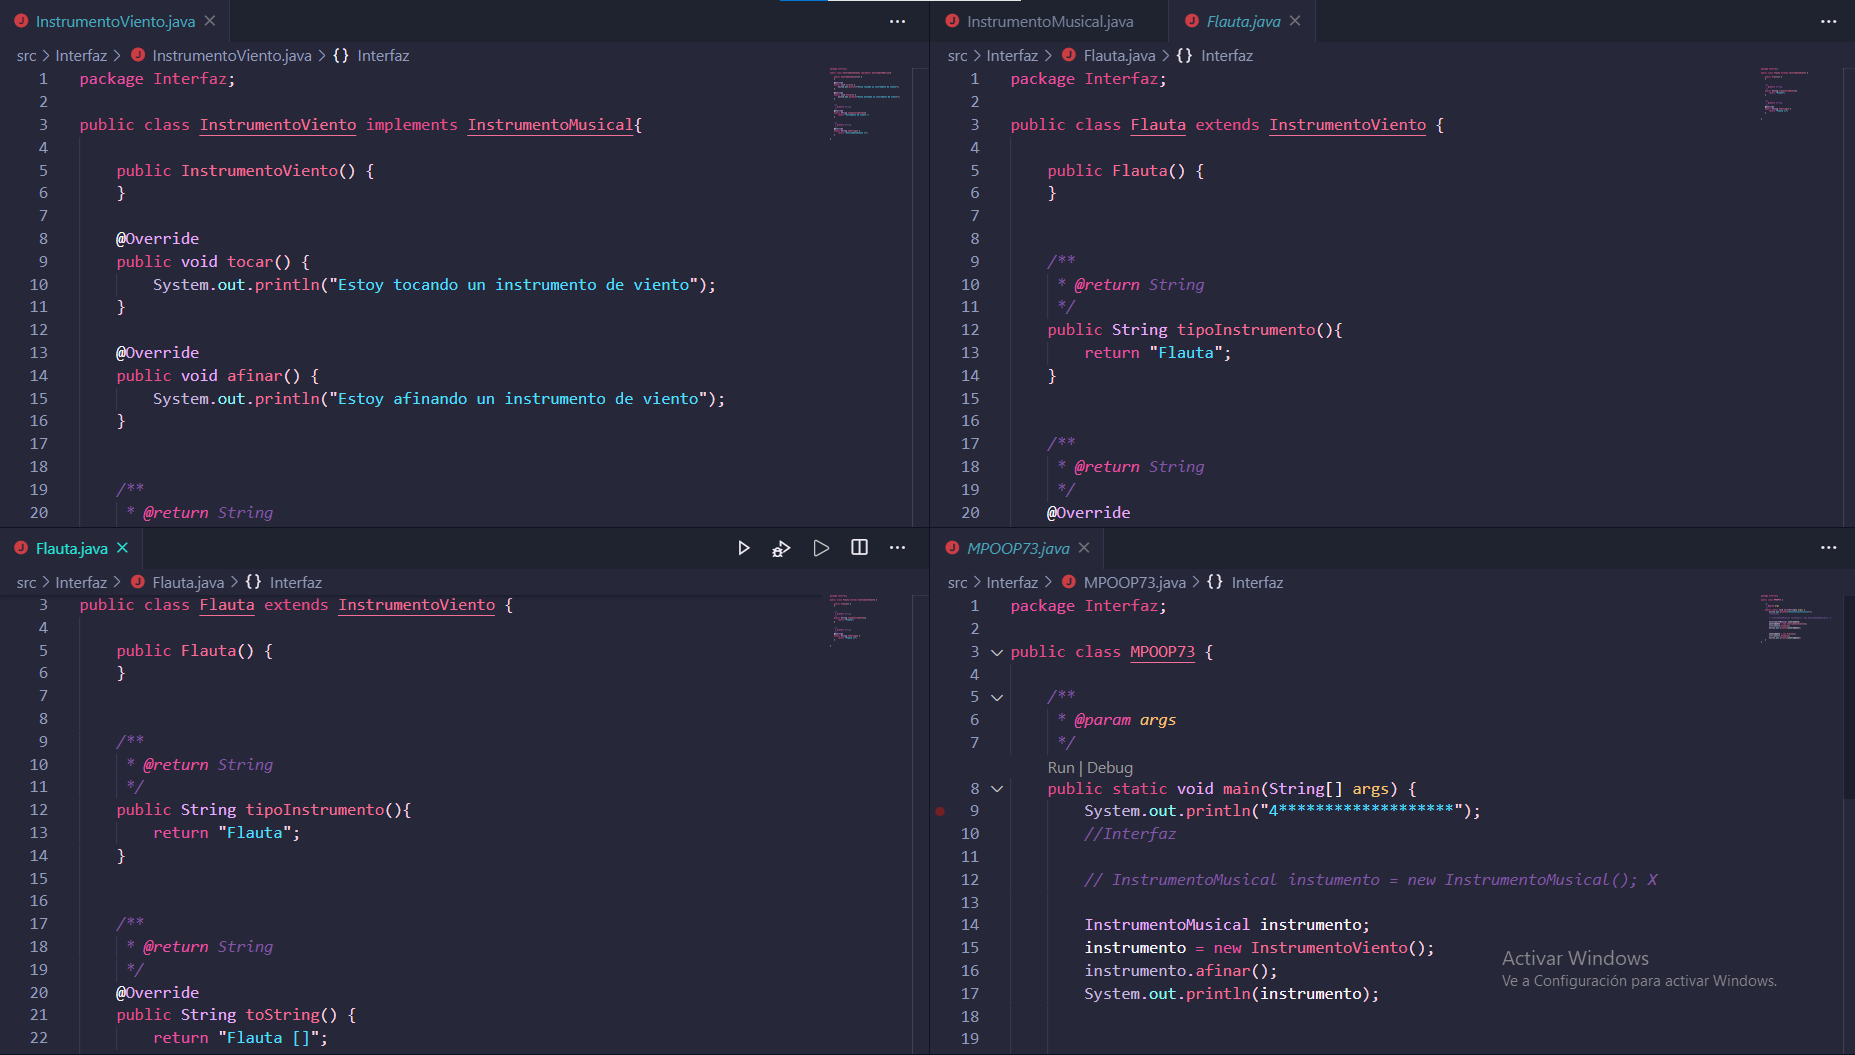
\includegraphics[scale=0.18]{./pics/8}}
            \caption{Clases que componen la paquetería interfaz.}
            \label{fig8}
        \end{figure}

        \subsection{Actividad cuatro}

        Para el ejemplo de las interfaces así cómo una clase, no es posible instanciar, por lo tanto hay que declararlo de la siguiente forma(Figura \ref{fig10})

        Es una especie de contenedor de variables y métodos que permiten mejor encapsulamiento, por lo tanto nivel de seguridad.

        \begin{figure}[htbp]
            \centerline{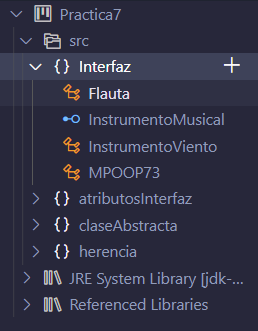
\includegraphics[scale=0.4]{./pics/13}}
            \caption{Jerarquía del paquete interfaz.}
            \label{fig9}
        \end{figure}

        Una interface puede ser el medio para operar datos y otras clases. 

        \begin{figure}[htbp]
            \centerline{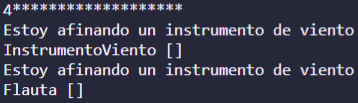
\includegraphics[scale=0.6]{./pics/14}}
            \caption{Actividad cuatro en consola}
            \label{fig10}
        \end{figure}

        Una interface también puede tener atributos.

    \section{Atributos de interfaz.}

        \subsection{Actividad cinco}

            Es sólo un ejemplo corto pero significativo:

            \begin{figure}[htbp]
                \centerline{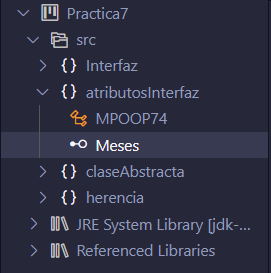
\includegraphics[scale=0.6]{./pics/11}}
                \caption{Jerarquía del paquete atributosInterfaz.}
                \label{fig11}
            \end{figure}

            Se usan por ejemplo nombres de los días del mes que se podría incluso para hacerlas en distintos idiomas.(Figura \ref{fig12})
            También podrían ser atributos para una interfaz gráfica, una skin para un personaje o incluso algoritmos de patrones en distintos tipos de poblaciones.
            \begin{figure}[htbp]
                \centerline{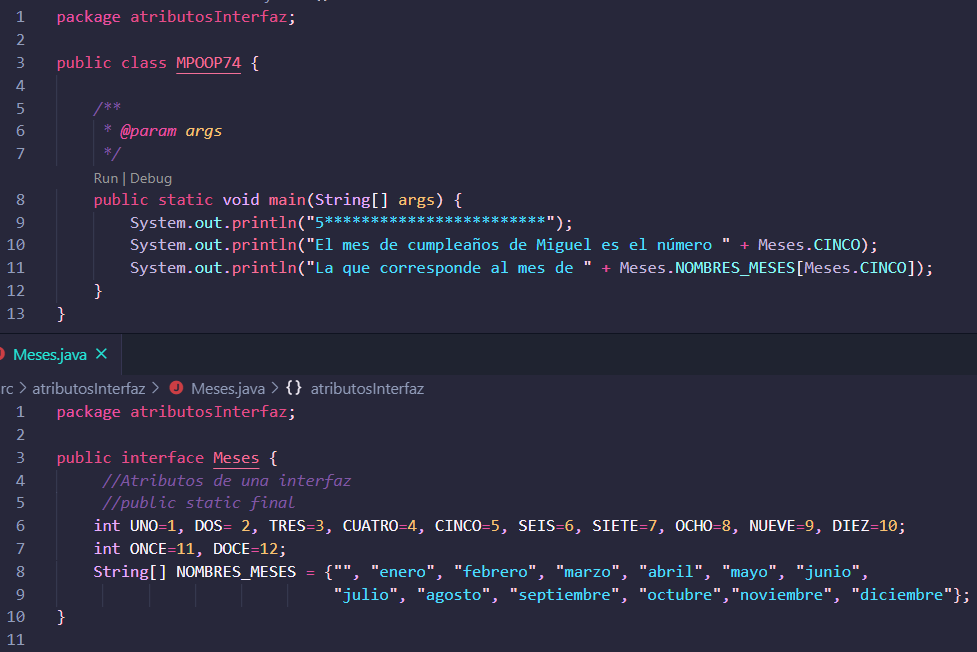
\includegraphics[scale=0.3]{./pics/15}}
                \caption{Main para actividad cinco e interfaz meses.}
                \label{fig12}
            \end{figure}



            \begin{figure}[htbp]
                \centerline{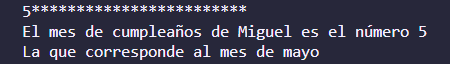
\includegraphics[scale=0.6]{./pics/12}}
                \caption{Actividad cinco en consola.}
                \label{fig13}
            \end{figure}
    \section{Conclusiones.}
        
        \subsection{Polimorfismo.}

            Entendemos que cada superclase puede crear instancias pero no viceversa.
            Por lo tanto de infiere que cada superclase se puede comportar cómo una subclase.

        \subsection{\texttt{instanceof}}

            El método \texttt{instanceof} devuelve las intancias de clases

        \subsection{\texttt{abstract} y \texttt{private}}

            Las diferencias entre una clase \texttt{abstract} y una \texttt{private} es que una se puede instanciar, mientras las otras solo permiten atributos dentro de un concepto abstracto.

        \subsection{\texttt{interface}}

            Una interface es un pequeño modelo que permite el almacenamiento de variables y métodos para usar en distintsas clases.

    \section{Repositorios.}

            \begin{itemize}
                \item Github https://github.com/RhoKratos/MPOOP7
                \item Gitlab https://gitlab.com/jeroorez/practica7
            \end{itemize}
    
    \medskip{}

    \bibliographystyle{./bibliography/IEEEtran}
    \bibliography{./bibliography/IEEEabrv,./bibliography/IEEEexample}
    
\end{document}